\paragraph{Creazione Domande}

\label{Creazione domanda vero/falso}

\begin{figure}[ht]
	\centering
	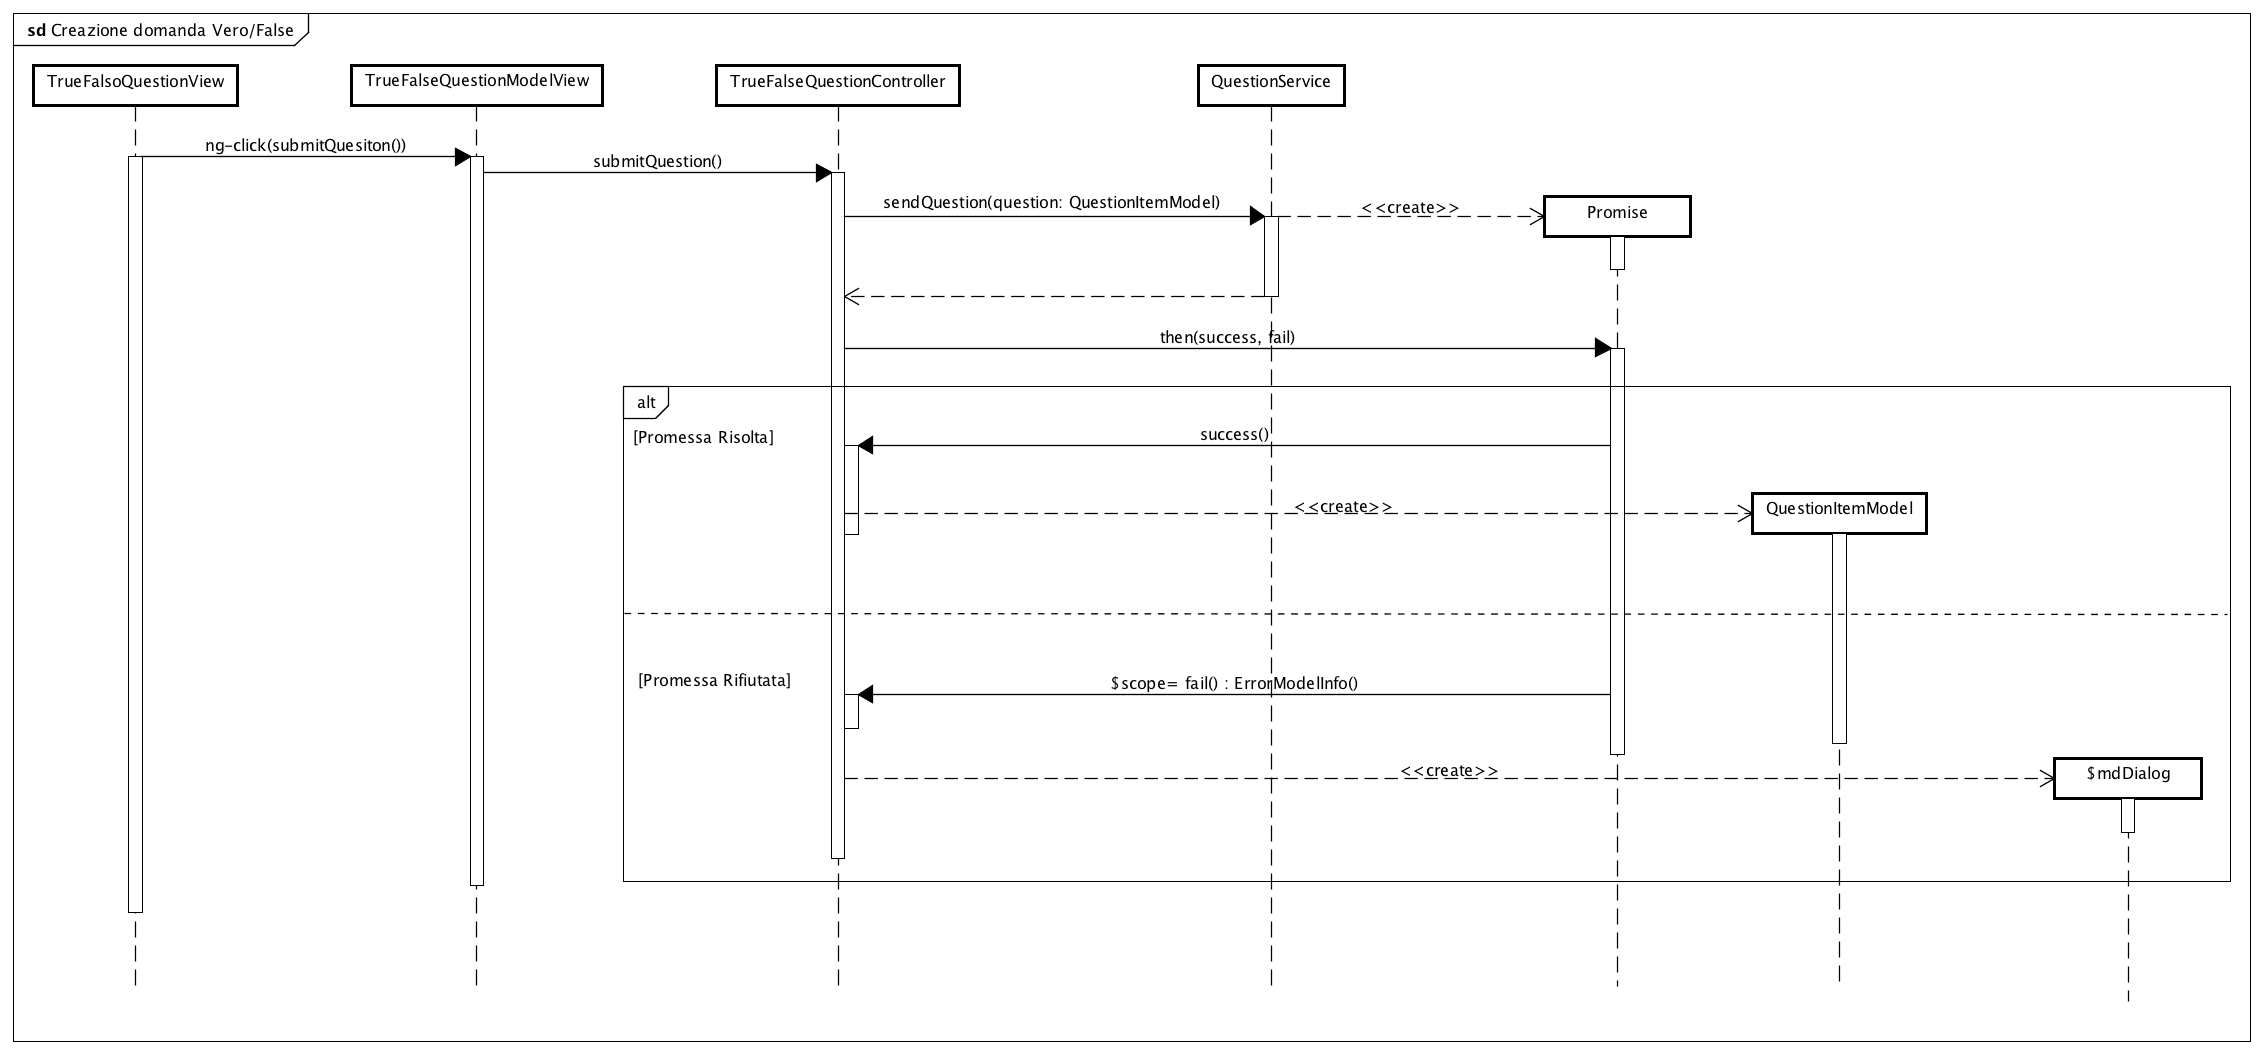
\includegraphics[scale=0.25,keepaspectratio]{UML/DiagrammiDiSequenza/Front-end/TrueFalseQuestionCreation.png}
	\caption{Creazione domanda vero/falso}
\end{figure} \FloatBarrier

Dopo che l'utente avrà selezionato il link di inserimento domanda, verrà richiamato il metodo del \texttt{controller\ped{G}} che richiederà al \texttt{service\ped{G}} l'inserimento della domanda tramite chiamata a risorse del back-end. Se la promessa creata dal \texttt{service\ped{G}} verrà accettata la domanda sarà inserita, altrimenti verrà restituito un oggetto contenente il testo dell'errore. \\ L'operazione sarà uguale per tutte le tipologie di domanda. 